\section{Datasets}

\subsection{Constellation Diagram Generation}

Constellation diagrams offer a more informative approach to modulation classification compared to raw time-series signals, capturing richer detail essential for accurate interpretation \cite{doan2020learning, 9289413}. The process of generating constellation diagrams for modulation signal classification involves multiple stages. We begin by mapping modulated signals onto a $7 \times 7$ complex plane, which provides sufficient space to capture signal samples while maintaining computational efficiency for SNR ranges of -10 dB to 10 dB. The basic constellation diagram is then enhanced through a multi-step process: first, as a gray image that handles varying pixel densities where multiple samples may occupy single pixels; second, as an enhanced grayscale image that employs an exponential decay model ($B_{i,j}$) to account for both the precise position of samples within pixels and their influence on neighboring pixels. This model considers the sample point's power ($P$), the distance between sample points and pixel centroids ($d_{i,j}$), and an exponential decay rate ($\alpha$) \cite{peng2018modulation}. To make the representation compatible with DenoMAE2.0, which expects RGB input, we generate a three-channel image by creating three distinct enhanced grayscale images from the same data samples, each utilizing different exponential decay rates. 

\subsection{Parameters in Sample Generation} %Dataset description add table

The dataset comprises signals from ten modulation formats, each originally of length $L_0 = 1024$. To conform to the transformer's input dimensions, signals undergo a two-step preprocessing: (1) reshaping to $\mathbf{S}_1 \in \mathbb{R}^{32 \times 32}$, and (2) interpolation to $\mathbf{S}2 \in \mathbb{R}^{224 \times 224}$. For formats with $L_0 > 1024$ (e.g., $L_\text{GMSK} = 8196$), signals are initially downsampled to $L_0$. To match the three-channel structure of constellation images $\mathbf{I} \in \mathbb{R}^{3 \times 224 \times 224}$, $\mathbf{S}_2$ is replicated across three channels, yielding $\mathbf{S}_3 \in \mathbb{R}^{3 \times 224 \times 224}$. All signals are sampled at $f_s = 200$ kHz, ensuring consistency across modulation formats.

\section{Experimental Results}

\subsection{Denoising Performance}

\begin{figure*}[htbp]
    \centering
    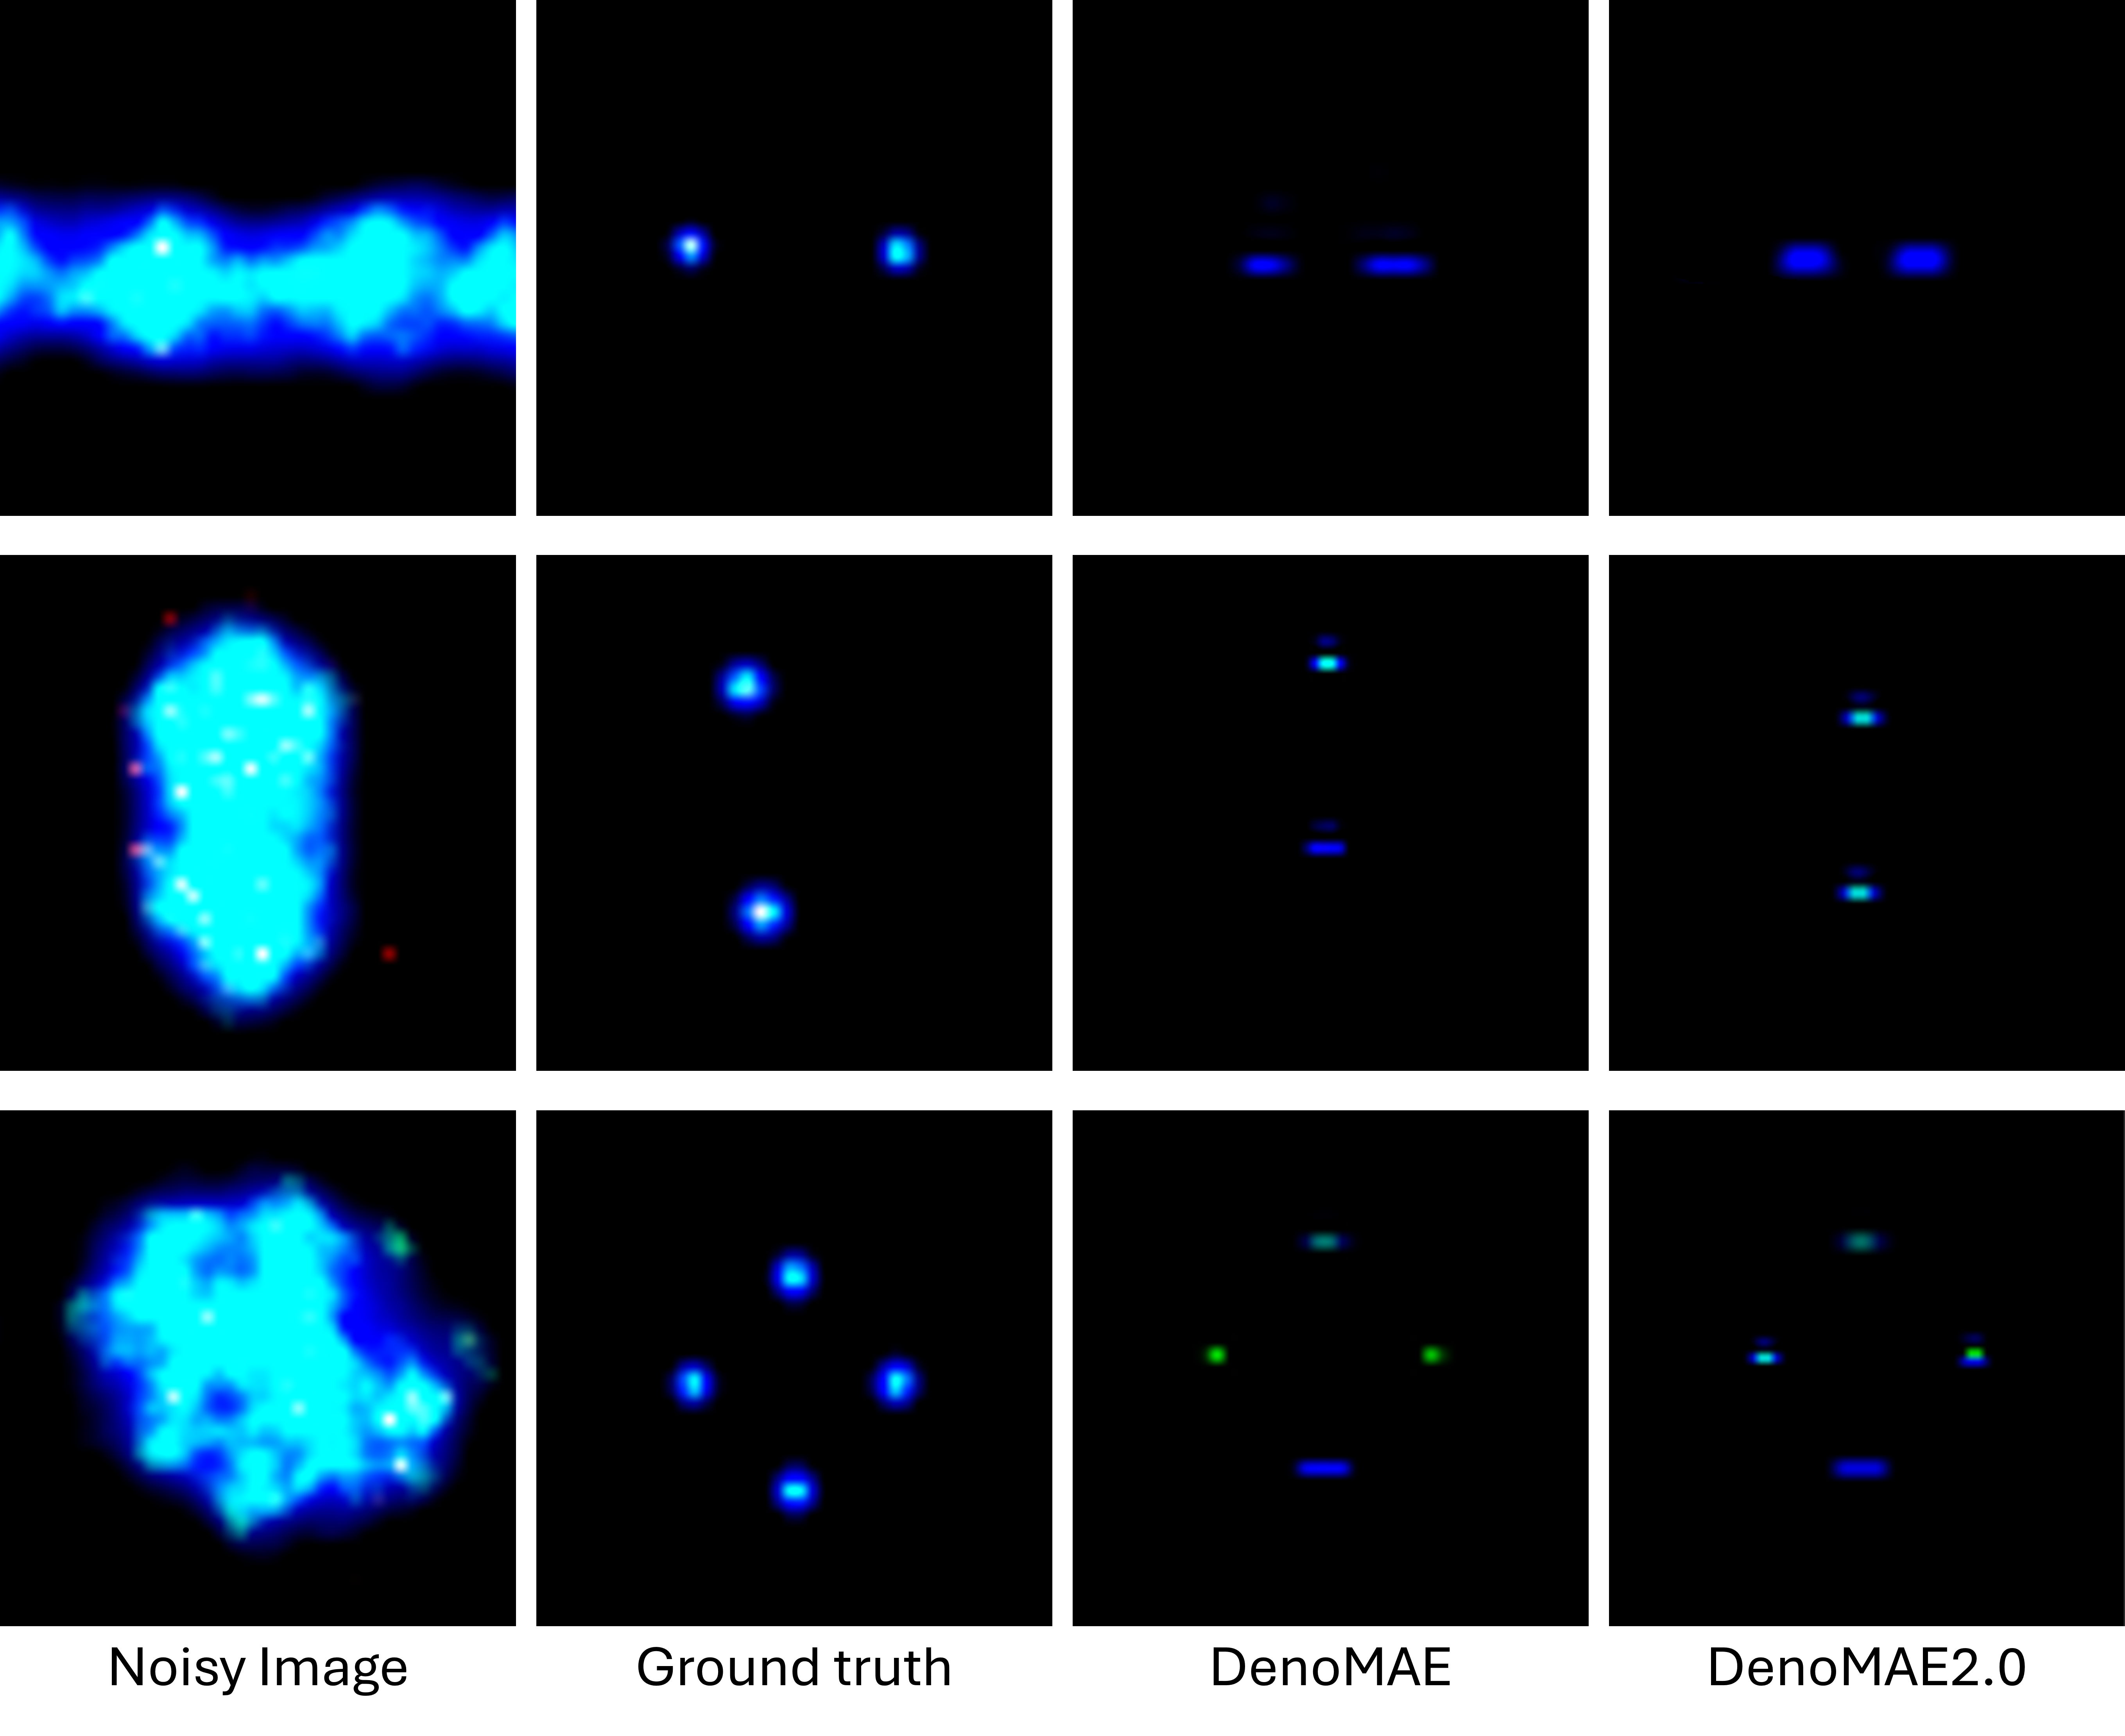
\includegraphics[width=0.7\linewidth]{images/recon.png}
    \caption{Reconstruction}
    \label{fig:recon}
\end{figure*}

The denoising effectiveness of DenoMAE2.0 is evident in the reconstructed constellation diagrams shown in Figure \ref{fig:recon}. Compared to DenoMAE, DenoMAE2.0 achieves superior noise reduction while preserving key signal features crucial for modulation classification. Table \ref{tab:ssim_psnr_comparison} quantifies this improvement using two standard metrics: structural similarity index (SSIM) and peak signal-to-noise ratio (PSNR). Interestingly, for the first image, DenoMAE achieved higher SNR and PSNR despite DenoMAE2.0 producing a visually superior reconstruction. However, for the remaining two samples, DenoMAE2.0 outperformed DenoMAE in both SSIM and PSNR (dB).

\begin{table}[htbp]
    \centering
    \renewcommand{\arraystretch}{1.2}
    \begin{tabular}{|c|c|c|c|}
        \hline
        Method & Image & DenoMAE & DenoMAE2.0 \\ \hline
        \multirow{3}{*}{SSIM} 
        & Image1 & 0.9660 & 0.9634 \\ 
        & Image2 & 0.9407 & 0.9607 \\ 
        & Image3 & 0.9422 & 0.9466 \\ \hline
        \multirow{3}{*}{PSNR (dB)} 
        & Image1 &  42.9054 & 42.3228 \\ 
        & Image2 & 42.0005 & 42.1061 \\ 
        & Image3 & 40.3067 & 40.7508 \\ \hline
    \end{tabular}
    \caption{Comparison of SSIM and PSNR for DenoMAE and DenoMAE2.0}
    \label{tab:ssim_psnr_comparison}
\end{table}

\section{Visualization with TSNE}

\todo[inline]{put tsne here}

\subsection{Finetuning Accuracy}

We compare DenoMAE2.0 with many of the state-of-the-art models to showcase its performance. As shown in Table \ref{tab:example}, DenoMAE2.0 achieves the highest test accuracy of 82.40\% among all compared methods. This represents a significant improvement over the baseline ViT (79.90\%) and other state-of-the-art approaches including DEiT (81.20\%), MoCov3 (81.00\%), BEiT (80.40\%), MAE (80.10\%), and the original DenoMAE (81.30\%). The consistent performance advantage demonstrates the effectiveness of our enhanced denoising strategy for effective representation learning during pretraining.

\begin{table}[htbp]
    \centering
    \resizebox{0.8\linewidth}{!}{%
    \begin{tabular}{|c|c|}
        \hline
        Method & Test accuracy (\%) \\ \hline
        ViT & 79.90 \\ \hline
        DEiT & 81.20 \\ \hline
        MoCov3 & 81.00 \\ \hline
        BEiT & 80.40 \\ \hline
        MAE &  80.10 \\ \hline
        DenoMAE &  81.30 \\ \hline
        DenoMAE2.0 &  \textbf{82.40} \\ \hline
    \end{tabular}%
    }
    \caption{Downstream accuracy.}
    \label{tab:example}
\end{table}

\subsection{Performance on Number of Epochs}

\begin{figure}[htbp]
    \centering
    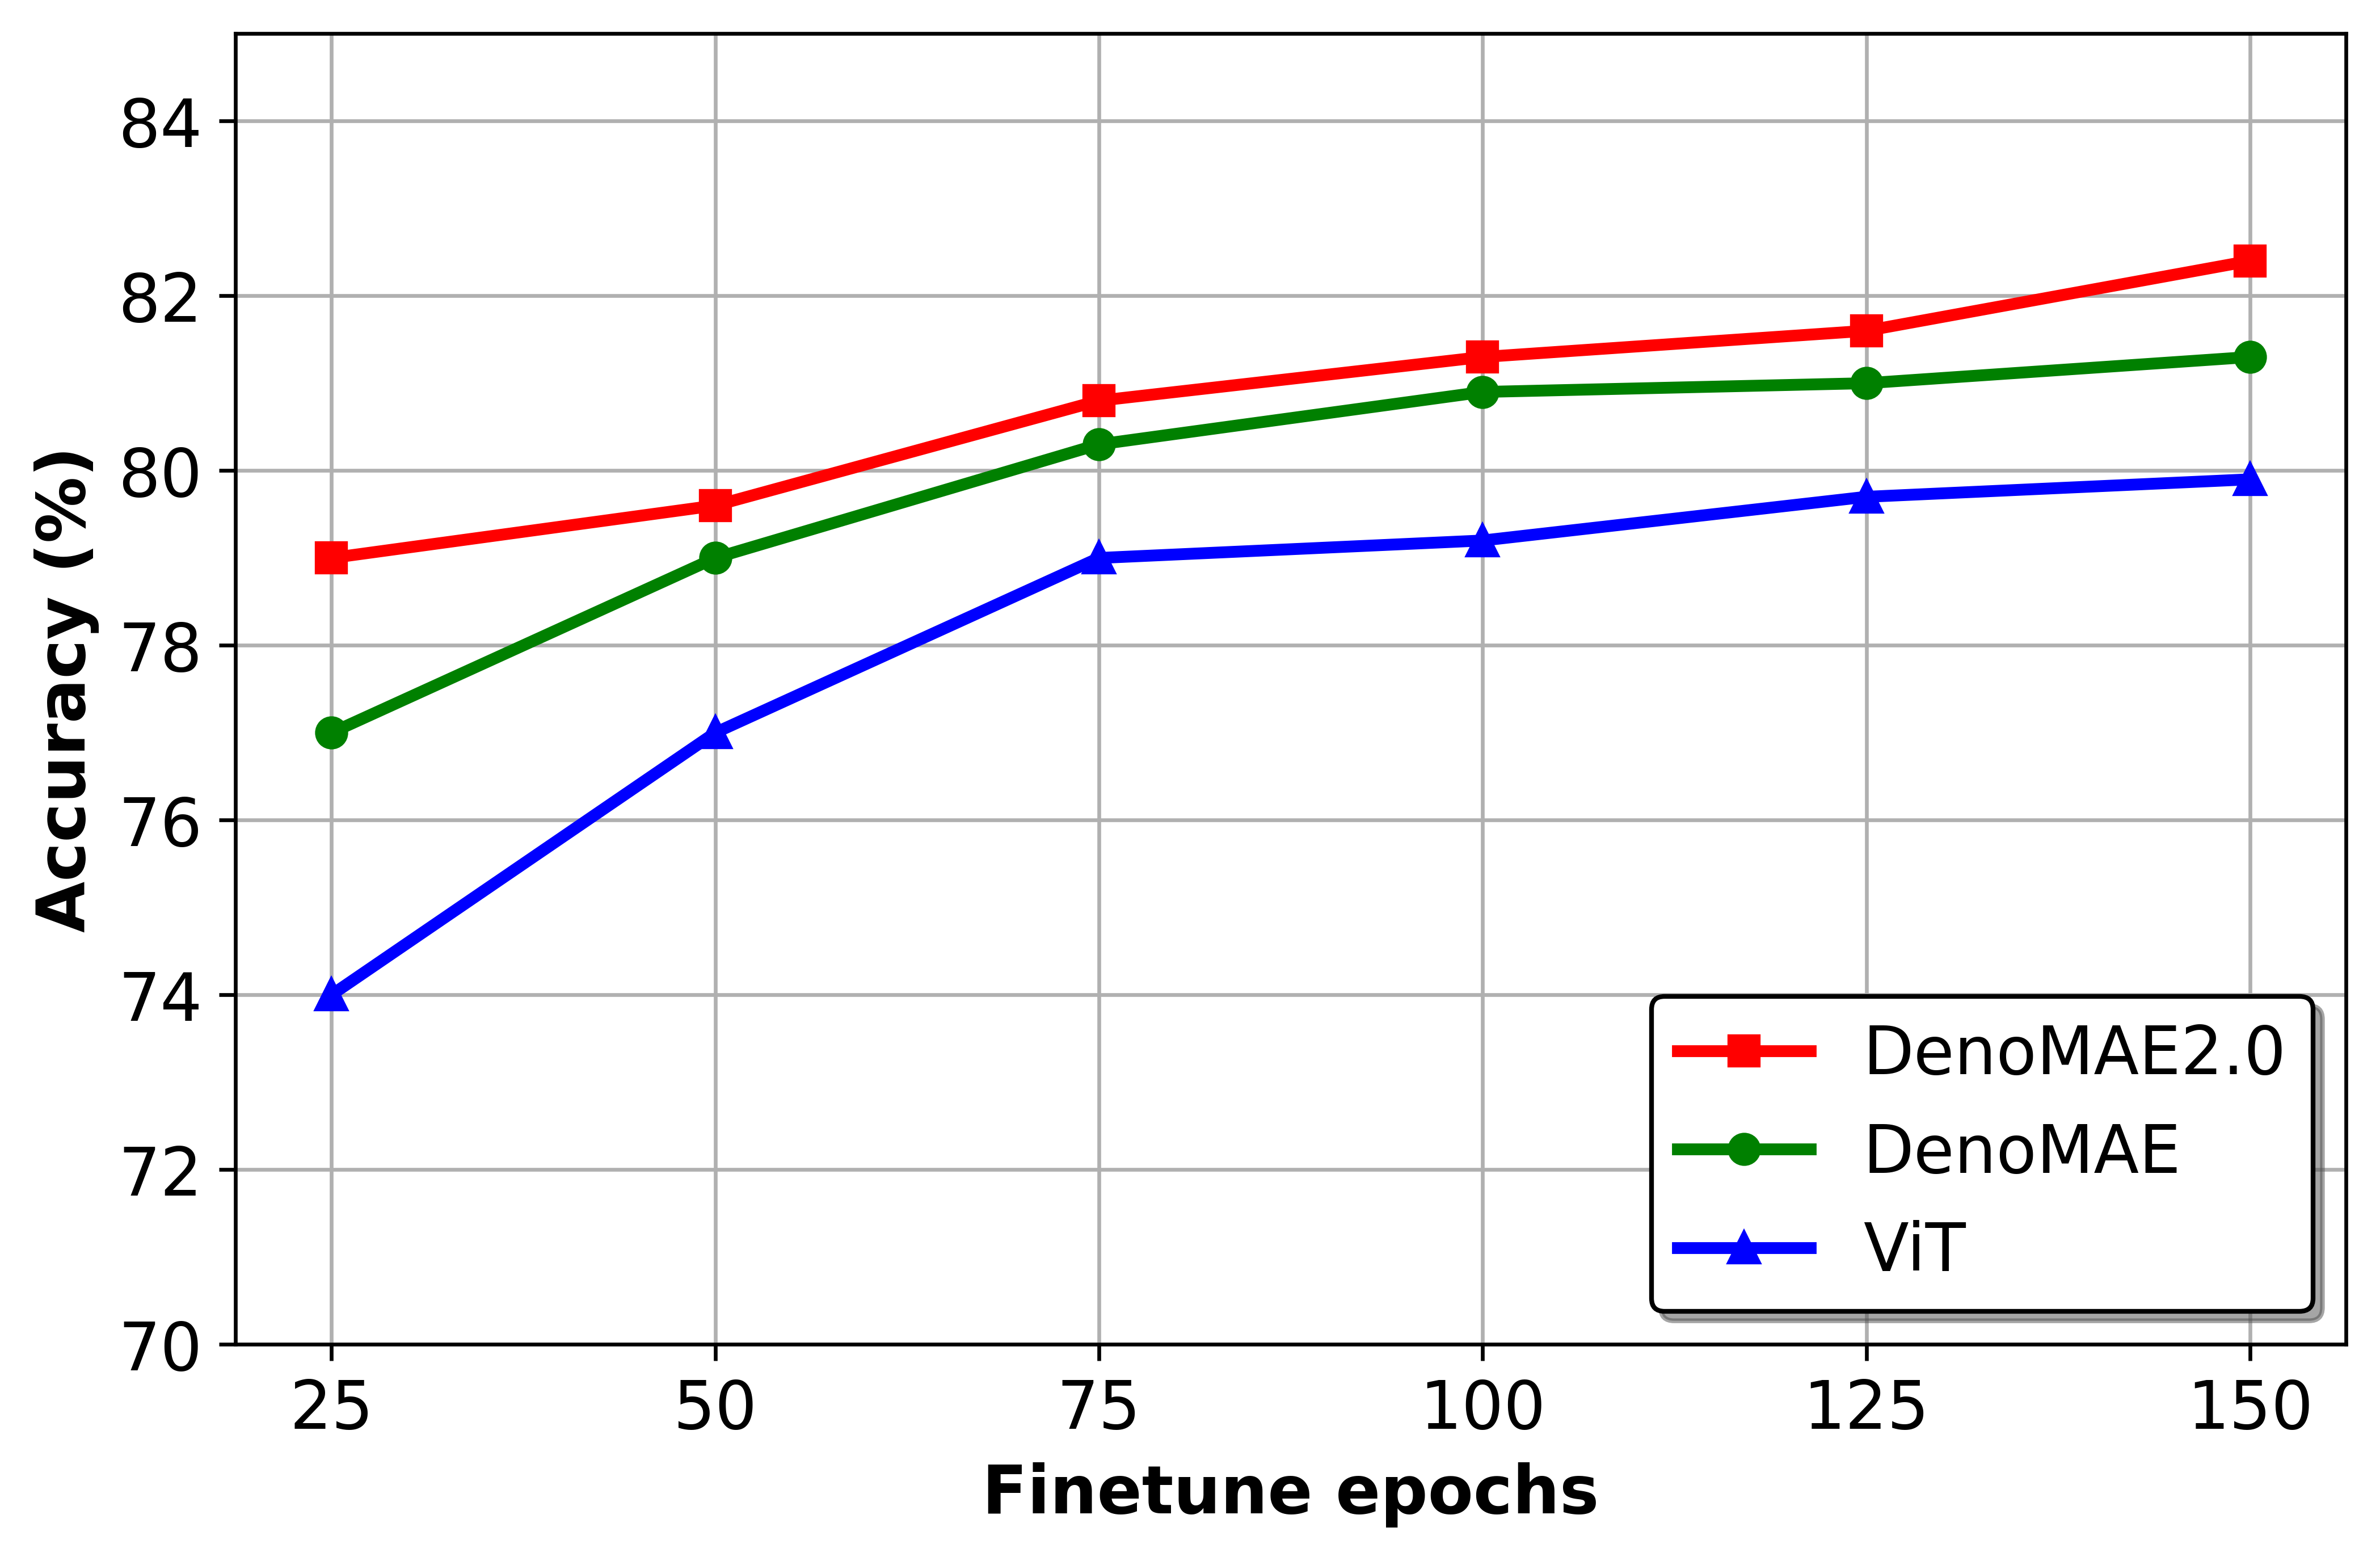
\includegraphics[width=0.9\linewidth]{images/finetune_epoch.png}
    \caption{Epoch finetuning.}
    \label{fig:epoch}
\end{figure}

Figure \ref{fig:epoch} illustrates the finetuning performance across different epochs. The plot shows a steady improvement in model accuracy as the number of epochs increases, with DenoMAE2.0 consistently outperforming baseline methods. DenoMAE achieves higher accuracy than ViT continuously. On the other hand, although the gap between DenoMAE and ViT is larger than DenoMAE and DenoMAE2.0, DenoMAE2.0 always obtains better accuracy than DenoMAE.

\subsection{Performance Across Different SNRs}

The SNR performance plot demonstrates robust classification accuracy across various SNRs ranging from -10 dB to 10 dB. As the SNR values increases all the methods perform better and when the SNR is low the performance degrades. ViT, which has no pertaining phase, presumably obntains the lowest performance in all cases. MAE, which pretrains on modulation signals but has no denoising capability, obtains a slight higher accuracy than ViT. DenoMAE obtains higher accuracy than MAE in most cases however for SNE of 2 and 3 we observe that MAE obtains higher accuracy. On the other hand, DenoMAE2.0 outperforms all the methods for all the SNRs.  Noteably, all the methods lose significant accuracy for snr lower than -2 dB. However, DenoMAE2.0 keeps on a comparatively acceptable accuracy till -7 db. All these outputs indicates DenoMAE2.0's superiority for a more effective representation and ropbustness.



\begin{figure}[htbp]
    \centering
    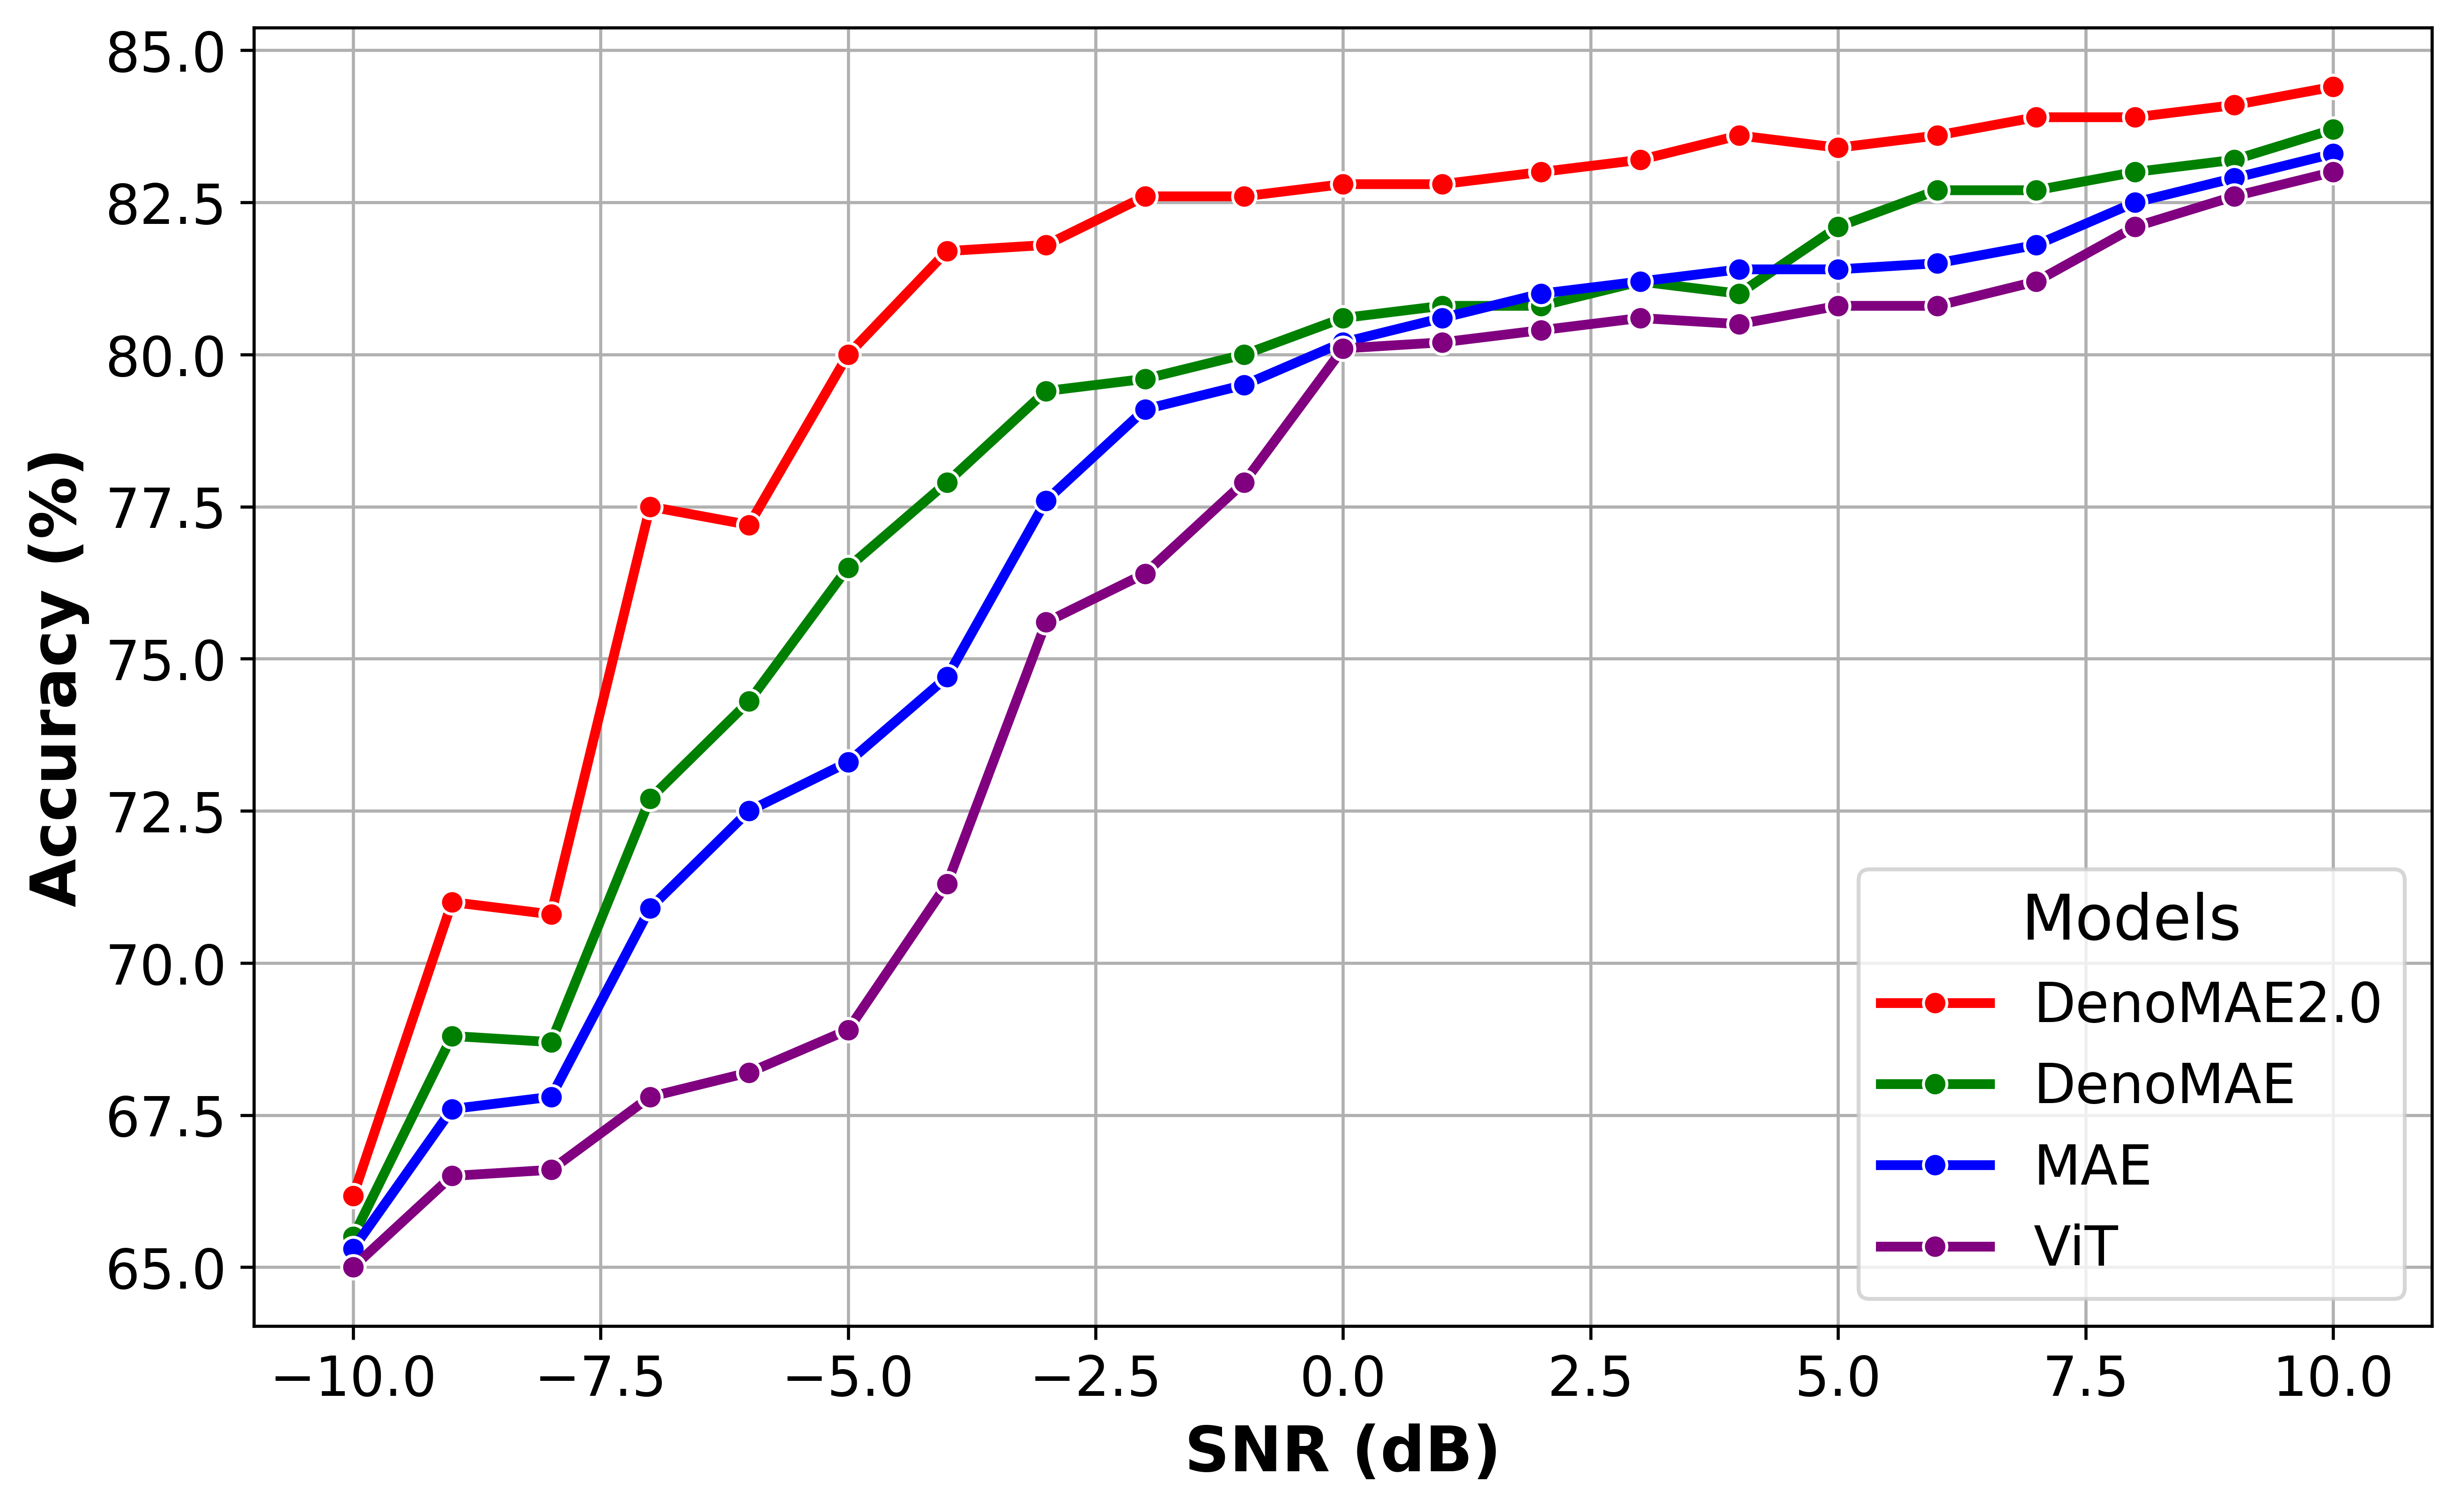
\includegraphics[width=\linewidth]{images/SNR_Accuracy_Plot.png}
    \caption{SNR}
    \label{fig:denomae2}
\end{figure}


\subsection{Transferability}

To show the transferability of DenoMAE2.0 on other similar task, we performed experiments on a similar benchmark dataset named RadioML. A brief description on the RadioML dataset is provided in the following subsection.

\subsubsection{RadioML Dataset}

RadioML 2018.01A \cite{o2018over} is a large-scale dataset designed for automatic modulation classification (AMC) and machine learning-based RF signal processing. It consists of 2,555,904 IQ (in-phase and quadrature) signal samples, where each sample is represented as a 1024×2 array, capturing both in-phase and quadrature components. The dataset spans 24 modulation types, including digital and analog schemes such as BPSK, QPSK, 8-PSK, 16-QAM, AM, and FM, making it a comprehensive resource for signal classification tasks. Signals are generated under 26 distinct signal-to-noise ratio (SNR) levels, ranging from -20 dB to +30 dB in 2 dB increments, simulating real-world conditions affected by fading, interference, and channel noise. Each modulation type and SNR combination contains 4096 samples, ensuring a balanced distribution for model training and evaluation. The dataset, widely used as a benchmark in wireless communication and spectrum sensing research, facilitates advancements in deep learning-based modulation recognition, interference mitigation, and cognitive radio applications.

To keep a consistent same scale implementation, we used 100 samples in each class for the 24 classes in RadioML for training and 10 samples in each class for testing. Therefore, we used only 2400 samples for training and 240 samples for testing. As a result we only used 0.103\% of the total dataset. We only obtain SNRs of -20, -10, 0, 10, 20 dB to show performance across low and high SNRs, as well as interpolaribility. 

\subsubsection{Performance}

The transfer learning capabilities of DenoMAE2.0 are depicted in Figure \ref{fig:trans}. All the methods perform better as the SNR increases and DenoMAE2.0 outperforms all the methods for all the SNRs. DenoMAE2.0 achieves the highest accuracy of 33.75\% for 20 dB SNR where as the closest accuracy obtained by DenoMAE is 21.92\% for 20 dB SNR. This indicates a high accuracy gain of 11.83\% for DenoMAE2.0. Similartly, for SNR of 10 dB, DenoMAE2.0 obtains an accuracy of 29.88\% where as the closest accuracy obtained by DenoMAE is 13.33\%. This indicates a high accuracy gain of 16.55\% more for DenoMAE2.0. As the SNR  decreases and goes out of bound of our pretraining, that is -10 db and -20 db, ViT fails to obtain a meaningful accuracy, achieves only a accuracy of around pure chance (4.27\%) for 24 classes. DenoMAE achieves a slightly improved accuracy than pure chance. However, DenoMAE2.0 achieves a significant accuracy of 7.08\% for -10 db and 6.67\% for -20 db. Therefore, DenoMAE2.0 shows a significant improvement in transferability and robustness for similar tasks.

\begin{figure}[htbp]
    \centering
    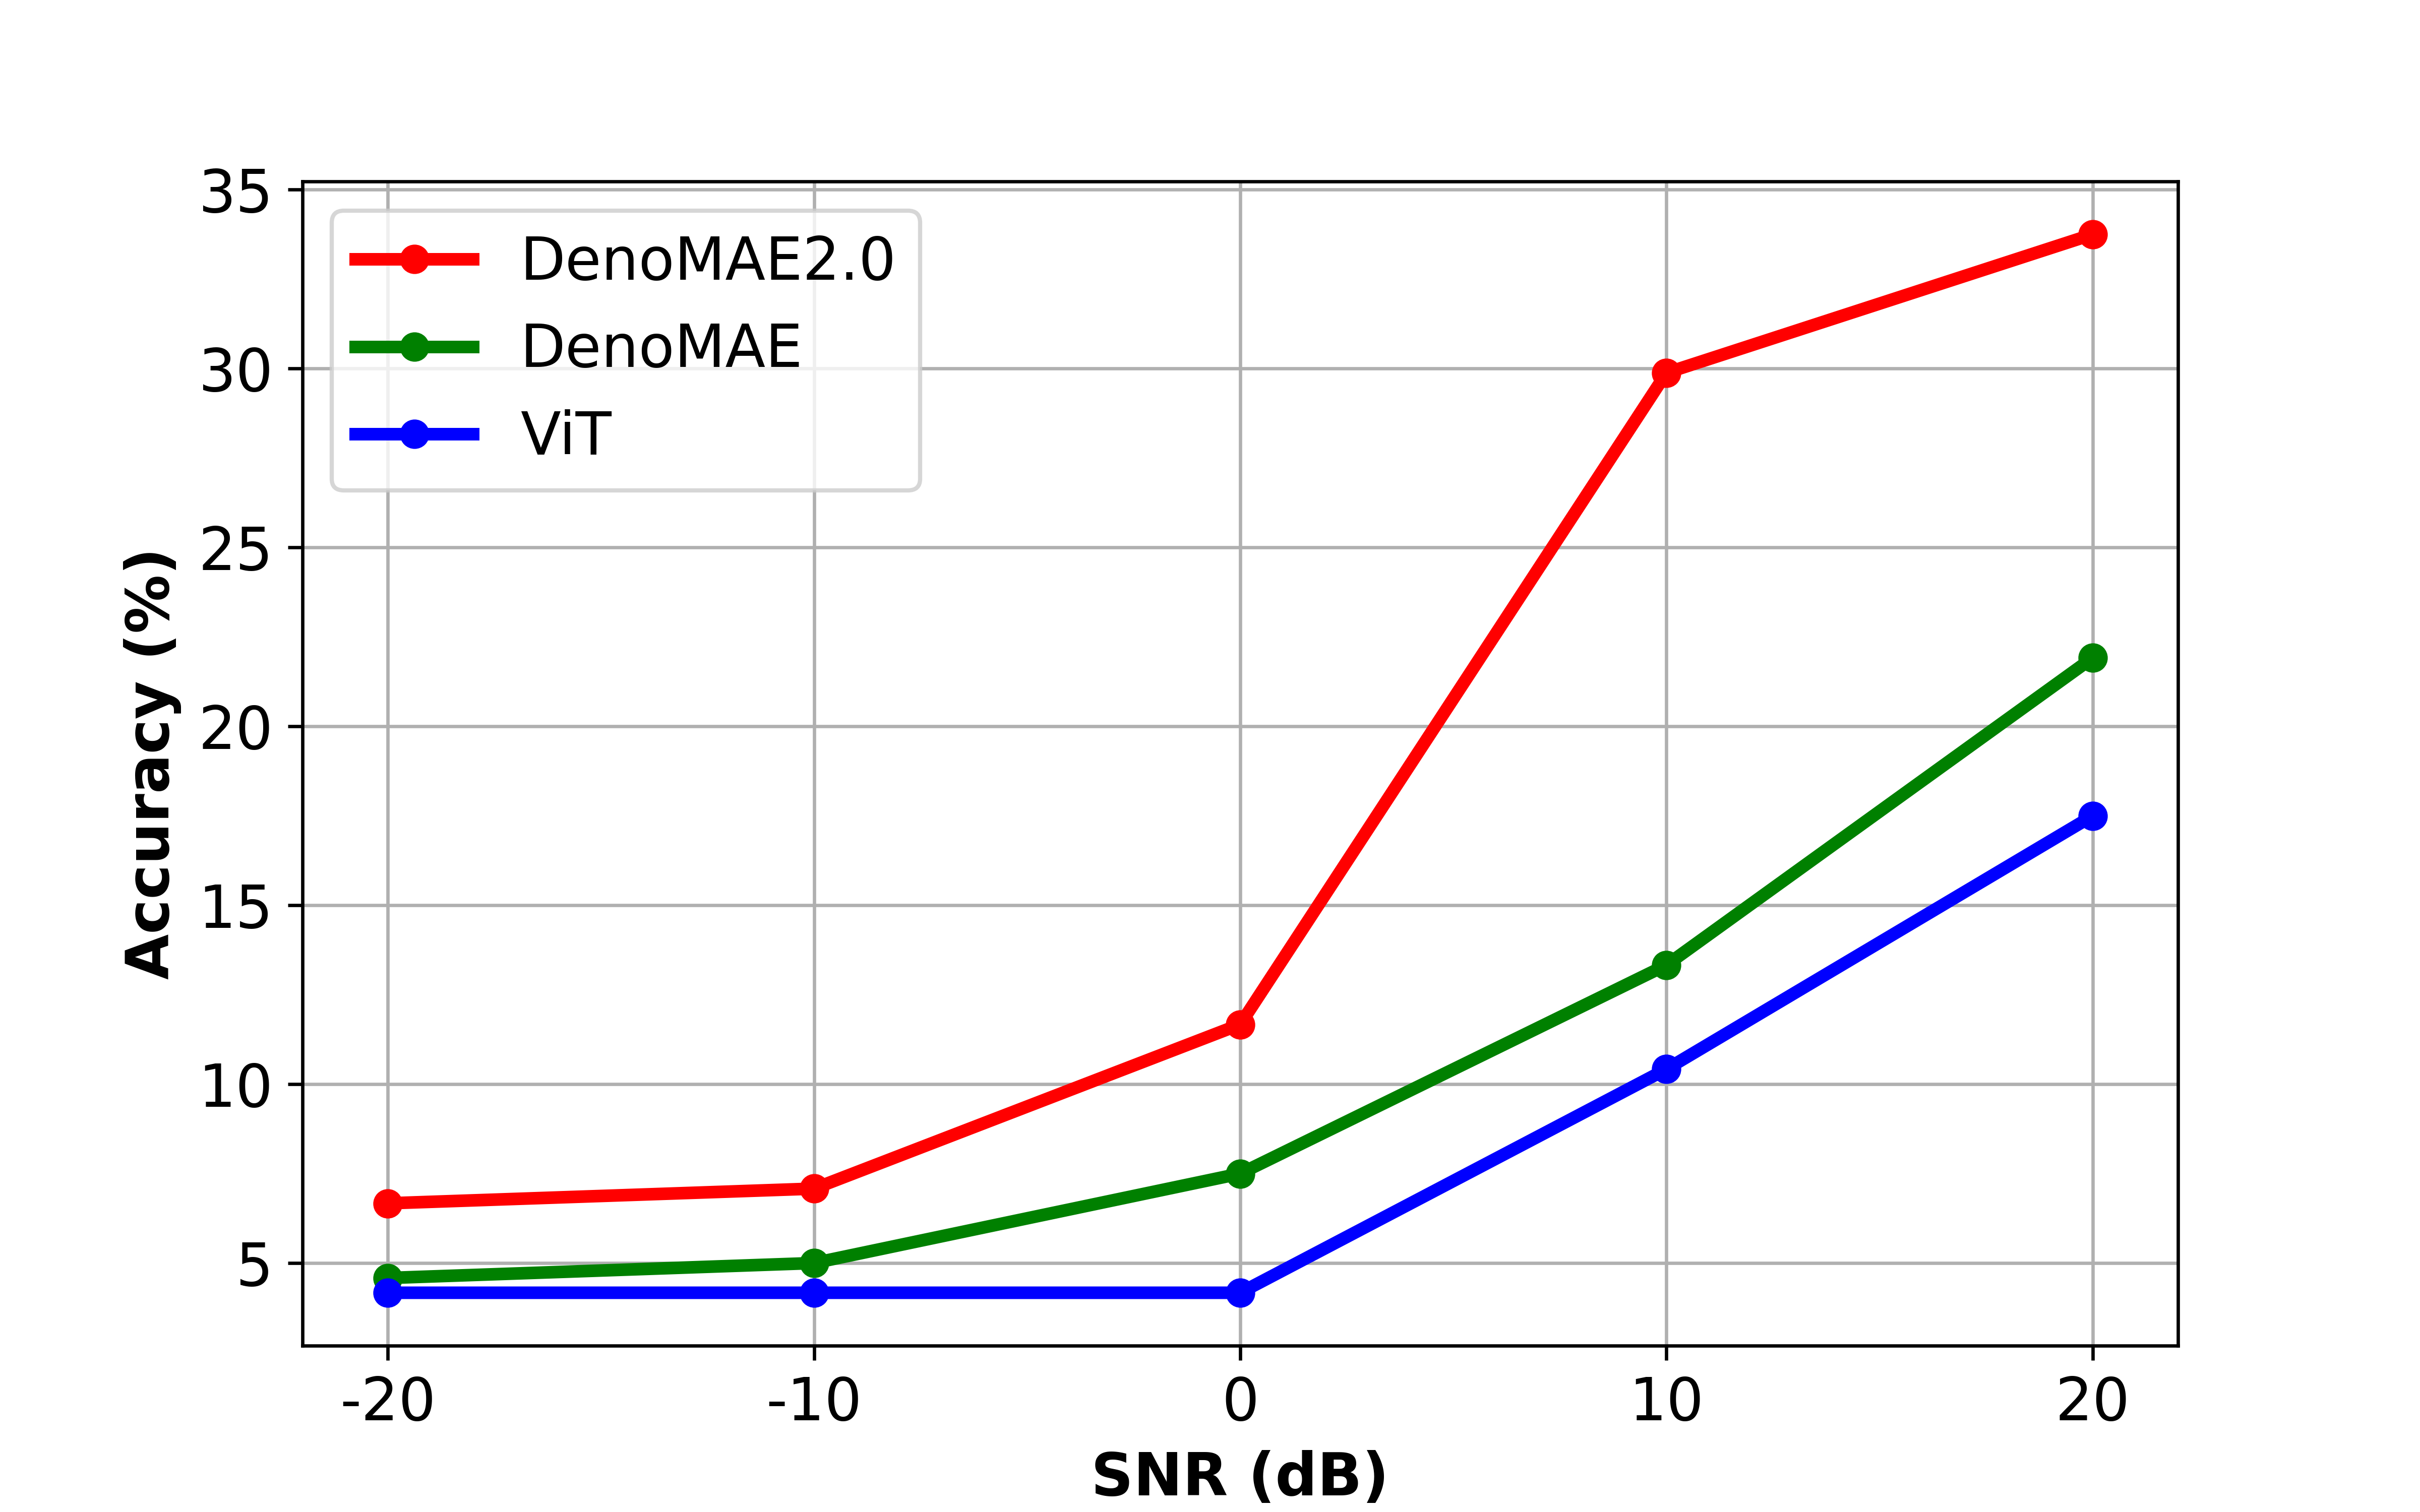
\includegraphics[width=\linewidth]{images/trans.png}
    \caption{Transfer}
    \label{fig:trans}
\end{figure}

